\begin{mdframed}[backgroundcolor=red!20, frametitlerulewidth=0pt, innertopmargin=-2mm, innerbottommargin=2mm, skipabove=0mm]

\section{Model Predictive Control MPC}
\end{mdframed}
\subsection{MPC and Tracking MPC}
\begin{minipage}{0.33\textwidth}
    \begin{tcolorbox}[colframe=green!50!black, colback=green!5!white, title=Pros, left=0.5mm, right=0.5mm]
    \begin{itemize}[leftmargin=*]
        \item Optimal control law
        \item Guaranteed stability 
        \item Constraints
        \item Disturbance rejection via receding horizon
        \item LTI: parametrized OCP in $x_0$
        \item Markovian systems
    \end{itemize}
    \end{tcolorbox}
\end{minipage}
\begin{minipage}{0.33\textwidth}
    \begin{tcolorbox}[colframe=red!50!black, colback=red!5!white, title=Cons, left=0.5mm, right=0.5mm]
    \begin{itemize}[leftmargin=*]
        \item Linear system model
        \item Model accuracy 
        \item Computationally expensive \& need to happen in one time step (online)
        \item Discrete state space
        \item Steady-state error
        \item Input disturbances, process noise, multiplicative noise
    \end{itemize}
    \end{tcolorbox}
\end{minipage}
\begin{minipage}{0.33\textwidth}
    \begin{tcolorbox}[colframe=gray!50!black, colback=gray!5!white, title=Examples, left=0.5mm, right=0.5mm]
    \begin{itemize}[leftmargin=*]
        \item Reference tracking
        \item Cruise control, autonomous driving
        \item Planning tasks
    \end{itemize}
    \end{tcolorbox}
\end{minipage}\\ \\
It is a static (memoryless), nonlinear (non-continuous), time-invariant feedback control law. \\
It is computed by solving an optimization control problem (OCP) parametrized by the initial state $x_0$ (time-invariant) and uses a receding horizon (same horizon length).
\begin{alignat*}{2}
    \min_{u, x} \quad & \sum_{k=0}^{K-1} g_k(x_k, u_k) + g_K(x_K) &&\\
    \text{subject to} \quad & x_{k+1} = f(x_k, u_k), &&k = 0, \ldots, K-1 \\
    & x_0 = x &&\\
    & x_k \in \mathcal{X}_k, &&k = 0, \ldots, K \\
    & u_k \in \mathcal{U}_k, &&k = 0, \ldots, K-1 \\
    & {\color{orange}x(T) = x_{\text{terminal}}} && 
\end{alignat*}

\subsubsection*{\textcolor{black}{Considerations}}
\begin{itemize}
    \item Does not manage to solve every optimization problem (for example when the optimal input turns out to be a the end of the horizon and there is no terminal constraint).
    \item \begin{minipage}[t]{0.45\textwidth}
            \textbf{Offline computation of $u^\star_0(.)$}
            \begin{itemize}
                \item Extremely complex
                \item Abundant computation power
                \item Large memory requirement (store all trajectories)
                \item Example: unconstrained linear MPC: first element of finite-time LQR
            \end{itemize}
         \end{minipage}\hfill
         \begin{minipage}[t]{0.45\textwidth}
            \textbf{Online computation of $u^\star_0(.)$}
            \begin{itemize}
                \item Tractable
                \item Limited time 
            \end{itemize}
        \end{minipage}
    \item Tracking is achieved by a change of coordinates $\left\{
        \begin{aligned}
            &\tilde{x} = x - x_\mathrm{ss} \\
            &\tilde{u} = u - u_\mathrm{ss}
        \end{aligned}
        \right.$
        \begin{itemize}
            \item Change of variables is inconsequential for LTI systems.
            \item $x_\mathrm{ss}$ is derived by first principles or from offline \textbf{steady state optimization} computation.
        \end{itemize}
\end{itemize}

\subsubsection*{Finite Horizon}
Discrete time system $x(k + 1) = A x(k) + B u(k)$ equilibrium point are defined by fixed points $x^\star = A x^\star + B u^\star$.\\ \\
\textcolor{blue}{Lyapunov Stability for Discrete-Time}\\
Let $x^\star = 0$ and $V$ be a continuous function such that
\begin{itemize}
    \item $V(0) = 0 \text{ and } V(x) > 0, \; \forall x \neq 0$
    \item $\Delta V(x(k)) \triangleq V(f(x(k))) - V(x(k)) < 0, \; \forall x(k) \in \mathcal{D}$
    \item $V$ radially unbounded: $\|x\| \to \infty \Rightarrow V(x) \to \infty$
\end{itemize}
$\Rightarrow$ then the origin is $\textbf{globally asy. stable}$.

\subsubsection*{\textcolor{orange}{Terminal constraint}\textcolor{black}{: $x(T) = x_{\text{terminal}}$}}
\begin{minipage}{0.58\textwidth}
    \begin{align*}
        W(x_{k+1}) &= \min \sum_{s=k+1}^{k+K} g(x_\mathrm{ss}, u_\mathrm{ss}) \\
        &= \min \sum_{s=k}^{k+K-1} g(x_\mathrm{ss}, u_\mathrm{ss}) - g(x_k, u_k) + \cancel{g(x_{k+K}, u_{k+K})})\\
        W(x_{k+1}) &\leq W(x_k) - g(\tilde{x}_k, \tilde{u}_k) \leq W(x_k)
    \end{align*}

    \subsubsection*{\textcolor{black}{Considerations}}
    \begin{itemize}
        \item Stability can be lost when receding horizon is too short or when full state is not available.
        \item Other sufficient conditions to guarantee MPC stability
            \begin{itemize}
                \item Terminal cost function: $\phi(x(T))$
                \item Terminal constraint set: $x(T) \in \mathcal{X}_\text{terminal}$
                \item Large receding horizon $K$
            \end{itemize}
    \end{itemize}
\end{minipage}
\begin{minipage}{0.38\textwidth}
    \begin{figure}[H]
        \centering
        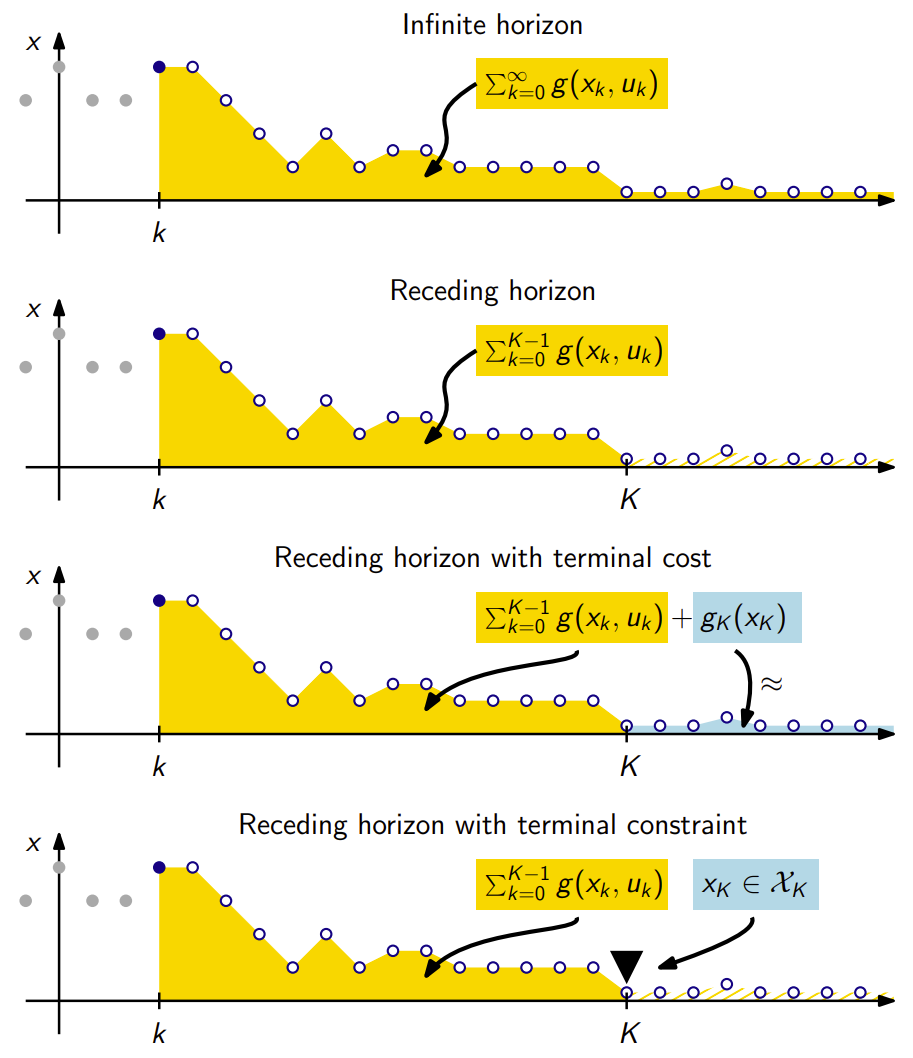
\includegraphics[width=0.9\columnwidth]{images/mpc.png}
    \end{figure}
\end{minipage}

\hrule

\subsubsection{Incremental MPC}
\begin{figure}[H]
    \centering
    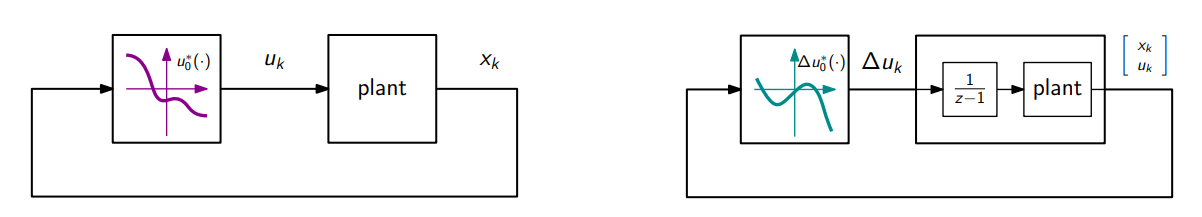
\includegraphics[width=0.8\linewidth]{images/incrementalMPC.png}
\end{figure}
\begin{minipage}[t]{0.48\textwidth}
    \textbf{Problems}:
    \begin{itemize}
        \item MPC will \textbf{not} achieve $x_\mathrm{ss}=0$ if a non-zero steady-state input is needed, because it inherently minimizes the input effort.
        \item Fragile against input disturbances, process noise, multiplicative noise.
        \item Low input can cause numerical issues.
    \end{itemize}
\end{minipage}
\begin{minipage}[t]{0.48\textwidth}
    \textbf{Solutions}:
    \begin{itemize}
        \item \textbf{Robustness}: Augment the plant with input integrator $\frac{1}{z-1}$ (if not present): more robust against disturbances and noise.
        \item \textbf{Numerical stability}: By penalizing $\Delta u_k = u_{k+1} - u_k$.
    \end{itemize}
\end{minipage}


\newpage

\subsection{Robust MPC}
\begin{minipage}{0.33\textwidth}
    \begin{tcolorbox}[colframe=green!50!black, colback=green!5!white, title=Pros, left=0.5mm, right=0.5mm]
    \begin{itemize}[leftmargin=*]
        \item Noise rejection ensuring feasible constraints
        \item Uncertainties within model
    \end{itemize}
    \end{tcolorbox}
\end{minipage}
\begin{minipage}{0.33\textwidth}
    \begin{tcolorbox}[colframe=red!50!black, colback=red!5!white, title=Cons, left=0.5mm, right=0.5mm]
    \begin{itemize}[leftmargin=*]
        \item Info about the noise/disturbance
        \item Open-loop: too conservative
        \item Closed-loop: difficult to find a parametrization
    \end{itemize}
    \end{tcolorbox}
\end{minipage}
\begin{minipage}{0.33\textwidth}
    \begin{tcolorbox}[colframe=gray!50!black, colback=gray!5!white, title=Examples, left=0.5mm, right=0.5mm]
    \begin{itemize}[leftmargin=*]
        \item Feasibility \& robustness: aerospace
        \item Reliability \& safety: driver assistant
        \item Power grids
    \end{itemize}
    \end{tcolorbox}
\end{minipage}\\ \\
\textbf{Problems:}
\begin{itemize}
    \item Cannot achieve zero tracking error due to the lack of an integrator.
    \item Neglected exogenous disturbances: \qquad $x_{k+1} = f(x_k, u_k, w_k)$
    \item Model mismatch: \qquad $x_{k+1} = \tilde{f}(x_k, u_k)$
    \item Missing dynamics / non-Markovianity: \qquad $
    \begin{cases}
        x_{k+1} = f(x_k, z_k, u_k) \\
        \textcolor{red}{z_{k+1} = f_z(x_k, z_k, u_k)}
    \end{cases}
    $
    \item Linearization: \qquad $x_{k+1} = \tilde{A}x_k + \tilde{B}u_k$
    \item And more: time discretization, quantization, time-varying parameters
\end{itemize}

\subsubsection{Disturbance Rejection in MPC}
\begin{figure}[H]
    \centering
    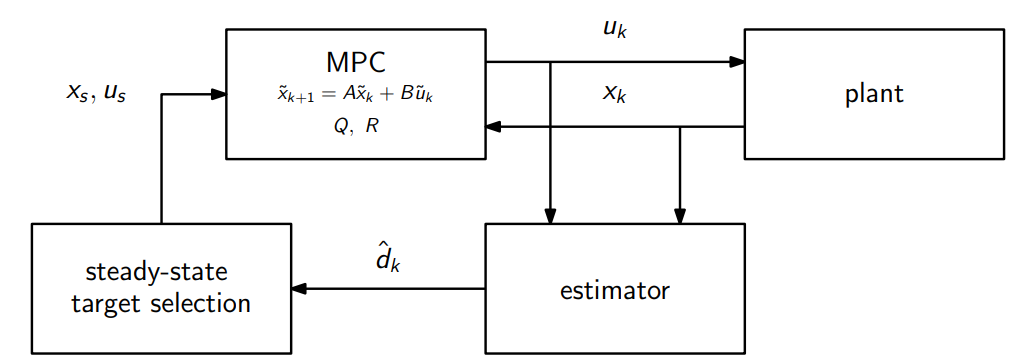
\includegraphics[width=0.6\linewidth]{images/distMPC.png}
\end{figure}
\textbf{Solutions:}
\begin{itemize}
    \item Model the disturbance as constant: \quad $\begin{bmatrix}
    x_{k+1} \\
    d_{k+1}
    \end{bmatrix}
    =
    \begin{bmatrix}
    A & B_d \\
    0 & I
    \end{bmatrix}
    \begin{bmatrix}
    x_k \\
    d_k
    \end{bmatrix}
    +
    \begin{bmatrix}
    B \\
    0
    \end{bmatrix}
    u_k$
    \item Predict of $x_{k+1}$ based on measurements $x_k, u_k$ and \textcolor{magenta}{estimate $\hat{d}_k$}: \quad $\hat{x}_{k+1} = A x_k + B u_k + \textcolor{magenta}{B_d \hat{d}_k}$
    \item Correct based on the prediction error: \quad $\hat{d}_{k+1} = \hat{d}_k + L \left( x_k - \hat{x}_k \right)$
    \item Select steady-state closer to specifications:
    \begin{align*}
    \min_{x_\mathrm{ss}, u_\mathrm{ss}} \quad & \| x_\mathrm{ss} - x_{\text{spec}} \|_{Q_\mathrm{ss}}^2 + \| u_\mathrm{ss} - u_{\text{spec}} \|_{R_\mathrm{ss}}^2 \\
    \text{subject to} \quad & \begin{bmatrix} I - A & -B \end{bmatrix} \begin{bmatrix} x_\mathrm{ss} \\ u_\mathrm{ss} \end{bmatrix} = \textcolor{magenta}{B_d \hat{d}_k} \\
    & x_\mathrm{ss} \in \mathcal{X} \\
    & u_\mathrm{ss} \in \mathcal{U}
    \end{align*}
\end{itemize}

\hrule

\subsubsection{Robust MPC}
\begin{minipage}[t]{0.48\textwidth}
\textbf{Closed-loop solution:}
\begin{itemize}
    \item Constructs a \textbf{feedback control} $u_1(x_1), \ldots, u_K^\star(x_K)$
    \item \textcolor{red}{Computationally intractable} (except for soft-constrained min-max LQR: worst-case scenario)
    \item \textcolor{ForestGreen}{Optimal}: all past information about the disturbance is used at each stage $k$
    \[
    \hat{w}_k = D^\dagger(x_{k+1} - A x_k - B u_k)
    \]
    \item \textbf{Dynamic programming} automatically returns the desired control law $u_0^\star(x)$ from offline computation.
    \item Corresponds to infinite-time optimal control at the limit $K \rightarrow \infty$.
\end{itemize}
\end{minipage}
\hfill
\begin{minipage}[t]{0.48\textwidth}
\textbf{Open-loop solution:}
\begin{itemize}
    \item Constructs an \textbf{input sequence} $u_0, u_1, \ldots, u_K$
    \item \textcolor{ForestGreen}{Computationally tractable} (convex optimization problem) but often \textbf{unfeasible}
    \item \textcolor{red}{Too conservative}: no past information about the disturbance is used except for the information available at $k=0$
    \item The desired control law $u_0^\star(x)$ is obtained by parametrizing the online optimization problem in $x$
\end{itemize}
\end{minipage}\\ \\

\hrule

\subsubsection{Feedback MPC}
A trade-off of the two solutions above: affine control law \quad $\boxed{u_k = v_k + Lx_k}$
\begin{itemize}
    \item $v_k$: Open-loop (feedforward) sequence/optimal policy
    \item $L$: Closed-loop (feedback) gain: rejects disturbances: \quad $x_{k+1} = (A+BL)x_k + Bv_k + Dw_k$
    \begin{itemize}
        \item $A+BL$ Hurwitz
        \item $L$ designed offline (can use Riccati by relaxing constraints of MPC)
    \end{itemize}
\end{itemize}
Alternative: optimize both $v$ and $L$ online $\rightarrow$ computationally complex $\rightarrow$ Tube MPC.

\newpage

\subsection{Economic MPC EMPC}
\begin{minipage}{0.33\textwidth}
    \begin{tcolorbox}[colframe=green!50!black, colback=green!5!white, title=Pros, left=0.5mm, right=0.5mm]
    \begin{itemize}[leftmargin=*]
        \item Considers complex metrics
        \item Efficient trajectories (transients)
        \item Linear program for linear $\ell$
        \item Future feasibility with steady-state terminal constraint
    \end{itemize}
    \end{tcolorbox}
\end{minipage}
\begin{minipage}{0.33\textwidth}
    \begin{tcolorbox}[colframe=red!50!black, colback=red!5!white, title=Cons, left=0.5mm, right=0.5mm]
    \begin{itemize}[leftmargin=*]
        \item More difficult to solve (not convex)
        \item Balancing economic objectives requires trade-offs
        \item Stability not guaranteed
    \end{itemize}
    \end{tcolorbox}
\end{minipage}
\begin{minipage}{0.33\textwidth}
    \begin{tcolorbox}[colframe=gray!50!black, colback=gray!5!white, title=Examples, left=0.5mm, right=0.5mm]
    \begin{itemize}[leftmargin=*]
        \item Efficiency tasks
        \item Processes: furnace, chemical industry
        \item Logistics, supply chain
    \end{itemize}
    \end{tcolorbox}
\end{minipage}\\ \\
It considers a \textbf{continuous} and \textbf{lower bounded} stage cost $\ell(x,u)$ (e.g. linear functions) that represents economic losses, energy use, cost of material, \ldots
\begin{align*}
    \min_{u, x} \quad & \sum_{k=0}^{K-1} \ell(x_k, u_k) \\
    \text{subject to} \quad & x_{k+1} = f(x_k, u_k), \quad k = 0, \ldots, K-1 \\
    & x_0 = x \\
    & x_k \in \mathcal{X}_k, \quad k = 0, \ldots, K \\
    & u_k \in \mathcal{U}_k, \quad k = 0, \ldots, K-1
\end{align*}
Alternative: \textbf{Steady-state optimization} problem and \textbf{tracking MPC} to follow reference:\\
\begin{minipage}[t]{0.48\textwidth}
    \textbf{\textcolor{LimeGreen}{Advantages}}
    \begin{itemize}
        \item Easier to use $\ell(x,u)$
    \end{itemize}
\end{minipage}
\begin{minipage}[t]{0.48\textwidth}
    \textbf{\textcolor{red}{Disadvantages}}
    \begin{itemize}
        \item Suboptimal solution.
        \item Cost is not reduced during system transients.
        \item Does not respond efficiently to disturbances. (Traffic example: offline compute $x_\mathrm{ss}, u_\mathrm{ss}$, but if there's an incident, they do not adapt to the new situation.)
    \end{itemize}
\end{minipage}\\
% \subsubsection*{\textcolor{black}{Considerations}}
% \begin{itemize}
%     \item Alternatively: \textbf{\textcolor{ForestGreen}{easier}} to use $\ell(x,u)$ to solve the \textbf{steady-state optimization} problem and \textbf{tracking MPC} to track, \textbf{\textcolor{red}{but}}
%         \begin{itemize}
%             \item Suboptimal solution.
%             \item Cost is not reduced during system transients.
%             \item Does not respond efficiently to disturbances. (Traffic example: offline compute $x_\mathrm{ss}, u_\mathrm{ss}$, but if there's an incident, they do not adapt to the new situation.)
%         \end{itemize}
% \end{itemize}
\subsubsection*{Infinite Horizon}
\begin{itemize}
    \item Economic interpretation (continuous processes, long-term gains, \ldots).
    \item May not drive the system to an equilibrium (not necessarily a problem).
    \item \textcolor{ForestGreen}{Boundedness} is guaranteed by the constraints (feasible future trajectory).
    \item \textcolor{red}{Computationally} intense due to infinite horizon. 
\end{itemize}
\subsubsection*{Finite Horizon}
\begin{itemize}
    \item \textcolor{ForestGreen}{Computationally} tractable.
    \item \textcolor{red}{Unstable trajectories} can emerge: cheap trajectory now, expensive fix later.
    \item \textcolor{red}{Infeasibility} at the end of the control horizon. 
\end{itemize}
\subsubsection*{\textcolor{orange}{Terminal constraint}\textcolor{black}{: $(x_\mathrm{ss}, u_\mathrm{ss})$}}
\begin{itemize}
    \item \textcolor{ForestGreen}{Computationally} more tractable.
    \item \textcolor{ForestGreen}{Future feasibility}.
    \item \textcolor{orange}{Stability} is \textbf{not guaranteed} as it was for MPC because $\ell(x,u)$ is not minimized at steady state. Nonetheless, asymptotic stability is \textbf{not desired} when using EMPC, such that it produces trajectories that are \textbf{efficient and economical}  (also limit cycles/periodic orbits) and do not converge to an equilibrium, which exhibits a higher cost.
    \item Even in the case in which the system converges to the steady state, EMPC produces \textbf{efficient}  trajectories to the equilibrium (theorem).
\end{itemize}
\textcolor{red}{\textbf{Note}}: stronger conditions are required to guarantee asy. stability.